\subsection{Emails in privacy policies}
\label{sec:policy-emails}

Privacy regulation such as GDPR and CCPA requires contact information to be included in the privacy policies.
Moreover, privacy policies may provide email addresses for contact, complaints or data access requests.
In order to identify emails we first parsed the HTML of the main article (the output of the Readability script) using the Beautiful Soup Python library~\cite{beautifulsoup4} and extracted all links with the ``mailto’’ scheme.
We then extracted email addresses from policy text using a regular expression search, and made sure that the email address has an IANA approved top level domain~\cite{iana-tld}.


We extracted 639,004 email address instances (96,656 distinct email addresses) from 486,938 policy snapshots (65,907 distinct websites).

First appeared in our dataset in 2006, California State Department of Consumer Affairs's email address (dca@dca.ca.gov) is the most common email address by distinct number of websites it was found on. The email was found in 1,173 policy snapshots from 226 distinct websites.


\begin{figure}[h]
\centering
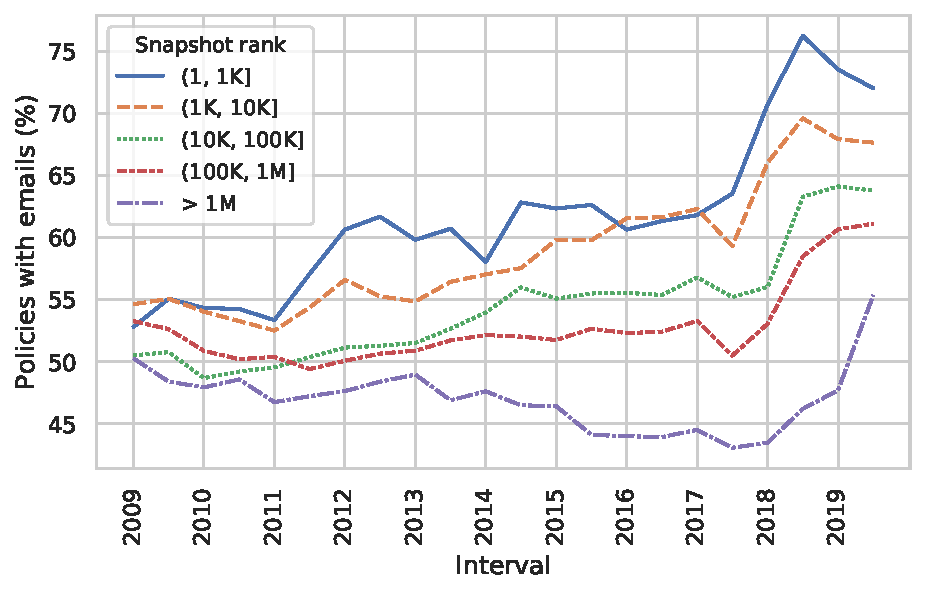
\includegraphics[width=0.99\columnwidth]{figures/lineplot_policies_with_emails_pct.pdf}
\caption{Percentage of privacy policies containing one or more email addresses per interval. }
\label{fig:pct-policies-with-emails}
\end{figure}


Figure~\ref{fig:pct-policies-with-emails} illustrates the percentage of policies
that contain one or more email addresses. Popular and recent privacy policy snapshots are more likely to contain email addresses.
Moreover, we note a 10\% increase (from 51.0\% to 60.6\%) in snapshots including email adresses between the second half of 2017 and 2019 -- before and after the GDPR came into effect. 

Analyzing the username (i.e. the local-part~\cite{email-local-part}) part of the email addresses,
we found a sharp increase in emails of the form 
privacy@... and dpo@... in the last two years, especially in the privacy policies of popular websites.
37.3\% of the policy snapshots in the 2019's second half has a privacy@ email,
up from 20.1\% in the second half of 2017 (85\% increase).
Similarly, only 0.5\% of the policies contained a dpo@... email in 2017's second half,
which raised to 8.3\% in two years.
